\documentclass{IEEEtran}
\usepackage{float}
\usepackage{graphicx}
\usepackage{booktabs}
\renewcommand{\baselinestretch}{1}
\setlength{\textheight}{9in}
\setlength{\textwidth}{6.5in}
\setlength{\headheight}{0in}
\setlength{\headsep}{0in}
\setlength{\topmargin}{0in}
\setlength{\oddsidemargin}{0in}
\setlength{\evensidemargin}{0in}
\setlength{\parindent}{.3in}
\newtheorem{hypothesis}{Hypothesis}
\newtheorem{nullhypothesis}{Null Hypothesis}
\usepackage{gensymb}


\begin{document}
\onecolumn


\section{Evaluation}

\subsection{Statistics}

The annotation table obtained from the image labelling is in the form of rectangle location and dimensions of the bounding box dimensions. The datasets are divided into three sets
\begin{enumerate}
\item \textit{Training Dataset}: annotation data obtained using the consumer drone and used for training the model.
\item \textit{Testing Dataset}: annotation data obtained using the consumer drone and used for testing the model.
\item \textit{GeoScience Dataset}: annotation data obtained using the data obtained from the GeoScience Department using a commercial drone.
\end{enumerate}

Bounding box heights, widths and aspect ratios can be obtained from the annotation data. The testing data and GeoScience data will be tested against the training data to see whether they are from the same population. If any populations are the same, the analysis done on one population should have the same evaluation results. If the populations are different, the analysis on both will be different, and the algorithms would need to be adapted to cater for this difference.

\subsubsection{Training Dataset}

Training bound boxes have a similar average width and average height pixel sizes. The average size is around 76 pixels, with minimum pixel size of around 28 pixels. The smallest bounding box matches the $32x32$ VGG16 pixel field of view within the \textit{conv5} output feature map. The highest number of bounding boxes fall under a $2x2$ VGG16 feature map.

\begin{table}[ht]
\caption{Consumer Drone Bounding Box Statistics - Train data}
\centering
\begin{tabular}{llllll}
       & Mean   & Std. Dev. & Min & Max & Population \\
Width  & 73.848 & 28.359 & 25 & 206  & 524 \\
Height & 79.293 & 27.197 & 31 & 207  & 524
\end{tabular}
\end{table}

\begin{figure}[h]
\centering
\label{consumerdronetrainhist}
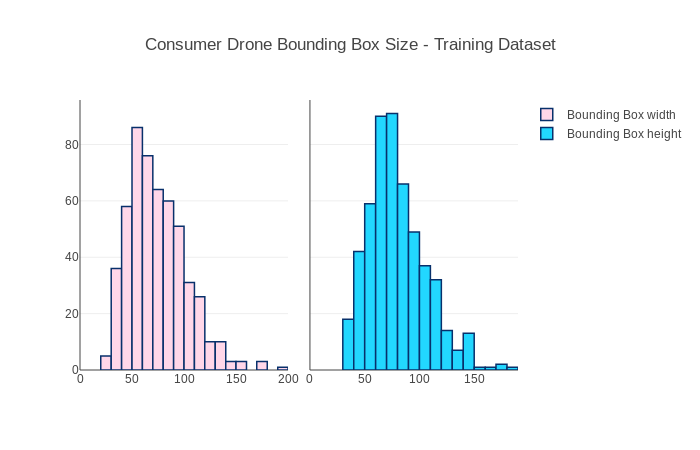
\includegraphics[scale=0.4]{images/train-histogram.png}
\caption{Consumer Drone Bounding Box Height and Width Histograms- Train data}
\end{figure}

As per qqplot show in figure \ref{consumerdronetrainqqplot} the data does not follow a normal distribution, so non-parametric tests will be performed to check that samples are obtained from the same population. 

\begin{figure}[h]
\centering
\label{consumerdronetrainqqplot}
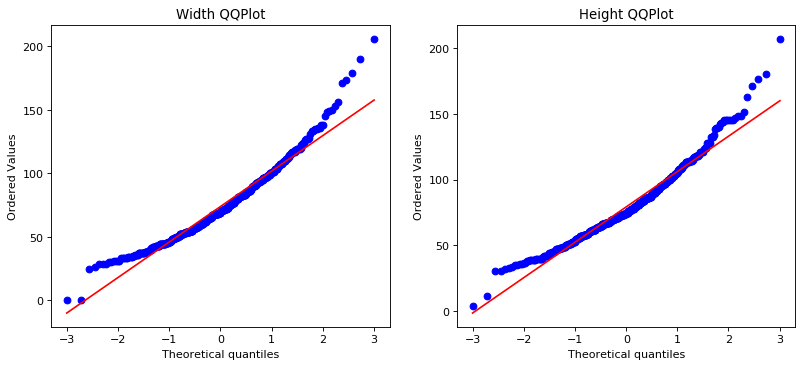
\includegraphics[scale=0.4]{images/train-qqplot.png}
\caption{Consumer Drone Bounding Box Height and Width QQplot - Train data}
\end{figure}

The aspect ratio of the training set as shown in the figure \ref{consumerdronetrainaspect} shows that there is no preference between log(-0.5) to log(0.5). This shows that there is no orientation preference of the bounding boxes in the training data set. As can be expected from aerial imagery data.

\begin{figure}[h]
\centering
\label{consumerdronetrainaspect}
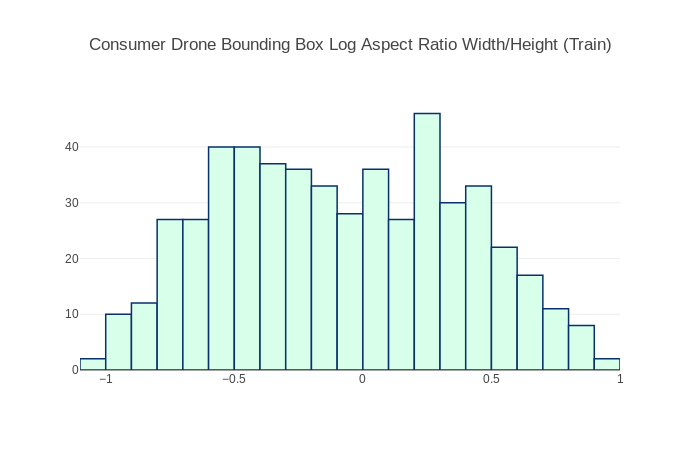
\includegraphics[scale=0.4]{images/train-aspect.png}
\caption{Consumer Drone Bounding Box Log Aspect Ratio Histogram - Train data}
\end{figure}

\subsubsection{Testing Dataset}

Testing bound boxes have a minor tendency to be larger in height than in width. The average size is also around 76 pixels, with minimum pixel size of around 29 pixels. Again this is within the field of view of the VGG16 pixel single feature vector of the \textit{conv5} output feature map. 

\begin{table}[ht]
\caption{Consumer Drone Bounding Box Statistics - Test data}
\centering
\begin{tabular}{llllll}
       & Mean   & Std. Dev. & Min & Max & Population\\
Width  & 71.654 & 29.435 & 26 & 199 & 246 \\
Height & 81.232 & 34.203 & 30 & 272 & 246
\end{tabular}
\end{table}

\begin{figure}[h]
\centering
\label{consumerdronetesthist}
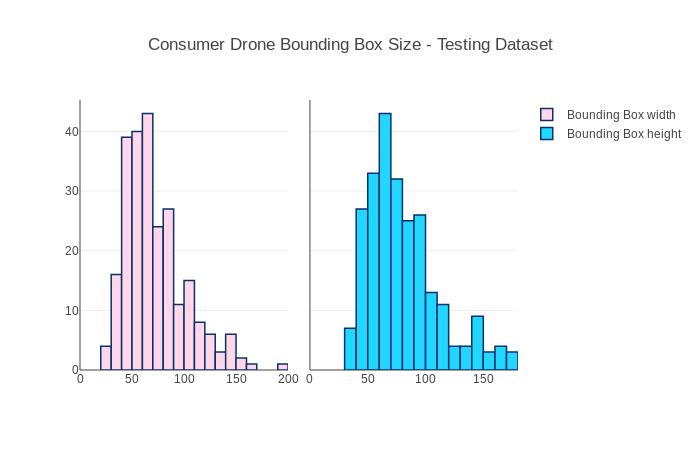
\includegraphics[scale=0.4]{images/test-histogram.png}
\caption{Consumer Drone Bounding Box Height and Width Histograms- Test data}
\end{figure}

As per qqplot show in figure \ref{consumerdronetrainqqplot} the data does not follow a normal distribution. This confirms the non-parametric tests to be performed on the population sampling.

\begin{figure}[h]
\centering
\label{consumerdronetestqqplot}
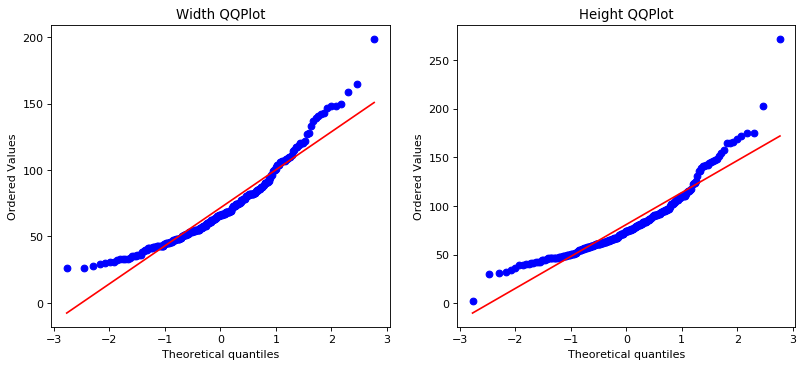
\includegraphics[scale=0.4]{images/test-qqplot.png}
\caption{Consumer Drone Bounding Box Height and Width QQplot - Test data}
\end{figure}

The aspect ratio of the training set as shown in the figure \ref{consumerdronetrainaspect} shows that there is no preference between log(-0.5) to log(0.5). This shows that there is no orientation preference of the bounding boxes in the training data set. The smaller values at the O for both the training set and the test set indicate that the objects bounding boxes are rarely a box shape (i.e. equal width and height) which indicates that the objects have an elongated shape. This is to be expected as the images labelled are of beverage bottles and containers, which are predominantly manufactured to be stacked side-by-side, and ergonomically designed to be handled by a single hand.

\begin{figure}[H]
\centering
\label{consumerdronetestaspect}
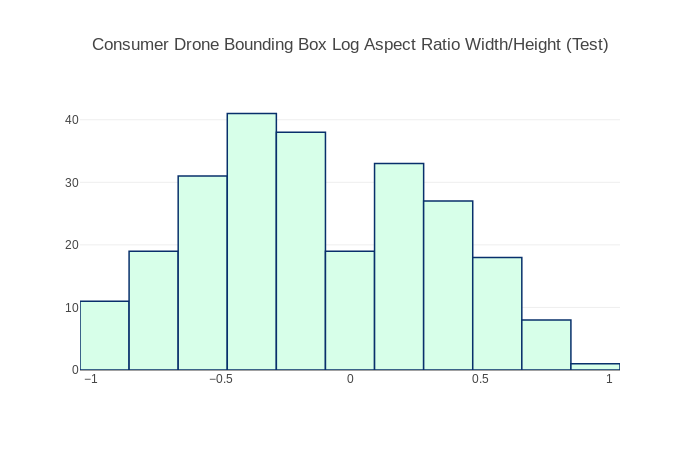
\includegraphics[scale=0.4]{images/test-aspect.png}
\caption{Consumer Drone Bounding Box Log Aspect Ratio Histogram - Test data}
\end{figure}


\subsubsection{GeoScience Dataset}

The Geoscience annotation also show no orientation prefernce with equal average width and height. The average size is also around 37 pixels, with minimum pixel size of around 11 pixels. This is a marked distinction from the previous datasets. The smaller bounding box sizes within this dataset might cause difficulties in the VGG16 field of view.

\begin{table}[ht]
\caption{GeoScience Drone Bounding Box Statistics - Data}
\centering
\begin{tabular}{llllll}
       & Mean   & Std. Dev. & Min & Max & Population\\
Width  & 36.038 & 11.921 & 11 & 120 & 793 \\
Height & 37.318 & 10.420 & 10 & 82 & 793
\end{tabular}
\end{table}

The average size of the bounding boxes of the GeoSciences is half that of the two other datasets. 

\begin{figure}[ht]
\centering
\label{geodronethist}
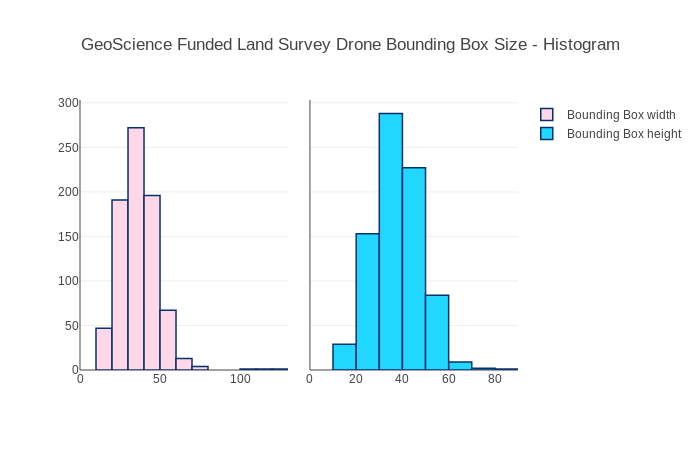
\includegraphics[scale=0.4]{images/geoscience-histogram.png}
\caption{GeoScience Bounding Box Height and Width Histograms}
\end{figure}

As per qqplot show in figure \ref{geodroneqqplot} the data does not follow a normal distribution. This confirms the non-parametric tests to be performed on the population sampling.

\begin{figure}[h]
\centering
\label{geodroneqqplot}
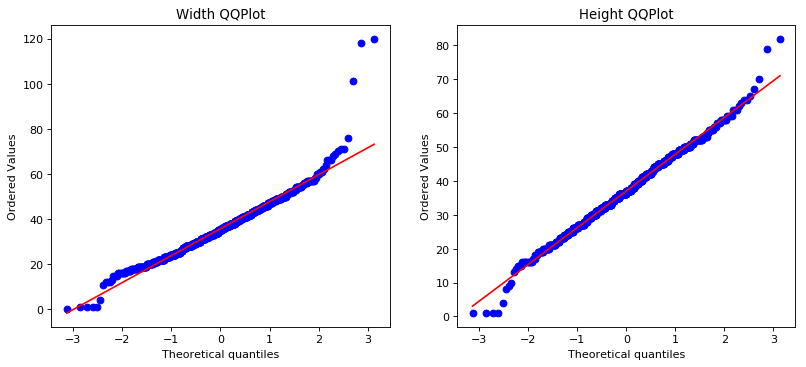
\includegraphics[scale=0.4]{images/geoscience-qqplot.png}
\caption{GeoScience Bounding Box Height and Width QQplot}
\end{figure}

The aspect ratio figure \ref{geodroneaspect} has a similar shape as the train and data set, confirming the nature of the images being labelled. 

\begin{figure}[ht]
\centering
\label{geodroneaspect}
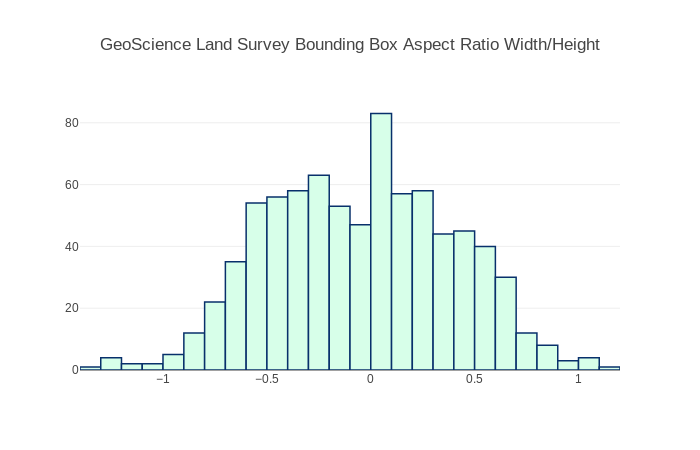
\includegraphics[scale=0.4]{images/geoscience-aspect.png}
\caption{GeoScience Bounding Box Log Aspect Ratio Histogram}
\end{figure}

\subsubsection{Population Testing}

The train, test and Geoscience population will be tested for independance. Since the populations are not normally distrbuted, a non-parametric test will be used. A two-tail Mann Whitney test will be performed. The whole data in the datasets will be used. The scale will be in pixel size. A confidence interval $\alpha = 0.05$ will be used.

The null hypothesis will be formulated :
\begin{nullhypothesis}
$H_0$: the distribution of the pixel sizes of the two datasets are equal
\end{nullhypothesis}
\begin{hypothesis}
$H_{A}$: the distribution of the pixel sizes is not equal
\end{hypothesis}

The two comparisons will be made between train vs test and train vs geoscience dataset.

\subsubsection{Train vs Testing Population}

Testing the two datasets using Mann Whitney results with U = 69299.00 and a p-value of 0.092 (for width) and U = 66246.50 and a p-value of 0.533 (for height) . Therefore we fail to reject the Null Hypothesis $H_0$. The train and testing data set come from the same population. This is to be expected as the data comes from the same sensor and using the same land-survey techniques.

\subsubsection{Train vs GeoScience Population}

Testing the two datasets using Mann Whitney results with U = 383029.00 and a p-value of 0.0 (for width) and U = 400391.50 and a p-value of 0.0 (for height) . Therefore we reject the Null Hypothesis $H_0$. The train and geoscience dataset come from the different populations. 

\subsubsection{Statistical Results}

The statistical tests show that the geoscience and the consumer drone data have different image sizes. This shows that the surveying techniques and parameters are different between geoscience data and consumer drone data. Comparing the geoscience images to that of the consumer drone, it can be deduced that the altitude of the surveys are different. This can also be the result of the drone operator knowledge of higher camera resolution.\newline

An algorithm which is dependant on the size of the picture for successful recognition, will have difficulty correctly infering the smaller sized dataset. The ability of the human labeller to correctly label the objects, indicates that the shape information is present. This has to be exploited by the CNN. The algorithm must be scale invariant or specifically tuned to the zoom levels of the geoscience dataset.\newline

\subsection{CNN Algorithm Testing}

Four CNN architectures will be testing for maximum validation accuracy results. The one with highest validation accuracy and highest foreground accuracy, precision and recall will be chosen. Each algorithm to be tested will be preloaded with algorithm weights pretrained on Imagenet. The fully connected layer at the end of the convolutional layers will be stripped off, and replaced by
\begin{enumerate}
\item A connected layer with softmax activation,
\item A connected layer with relu activation and a connected layer with softmax activation,
\item Two connected layers with relu activation and a connected layer with softmax activation
\end{enumerate}

The connected layer with softmax activation performs the two binary classifier between foreground and background. The connection layer between the Convolutional Layer and the Fully Connected Layer will be chosen from a Flatten layer, a Max Pooling Layer and a Global Average Pooling Layer. The layer used will depend on that specified by its relative academic paper when trained on the Imagenet database. If the training procedure does not converge, other layers will be tested.\newline

At this stage the trainable layers will be reserved only for the new fully connected layers. The best algorithm setup will be chosen. Further algorithm tuning will be performed by allowing more layers inside the convolutional blocks to be trained. Incremental training will be performed on previous trained models. Early Stopping will limit the epochs trained. \newline

\subsubsection{Dataset Preparation}

One dataset will be compiled for all tests. The dataset will consist of 
\begin{enumerate}
\item Plastic set available from the trashnet database \cite{Thung2017},
\item Plastic from the training set obtained from the Consumer Drone Survey,
\item 10 random background images obtained from the training set obtained from the Consumer Drone Survey,
\end{enumerate}
\par
The data will be fed using Keras ImageGenerator with inbuilt data augmentation algorithms. The options used for this testing are as follows:
\begin{enumerate}
\item Preprocessing Function: Keras provides algorithm specific preprocessing functions that transform an image to an output tensor of the same shape,
\item Shear range 0.2 : Angle of shear in degrees,
\item Horizontal Flip : Random horizontal flip of image,
\item Verticial Flip: Random vertical flip of image,
\item Zoom Range 0.2: Random zoom between 0.8 and 1.2 of the image size.
\end{enumerate}

All algorithms will have a default input tensor size of $224 x 224$. The fill-mode parameter is set to true so that no black areas appear within the image. Later RCNN tuning will test more data augment parameters and parameter ranges. \newline

Validation will only be preprocessed, but no augmentation of this set is performed.\newline


\subsubsection{Gradient Descent Optimizers}

RMSProp will be used for all the tests. The learning rate will be tuned according to the training and validation convergence speed. Convergence rate varies between 1e-4 to 1e-6.


\subsection{Algorithm Test Results}

\subsubsection{Inceptionv3}


\begin{enumerate}

\item: Inception with Max Pooling Layer, FCN 1-layer 1024 and Softmax Classifier


\begin{figure}[H]
\centering
\label{fig:incv3-sm}
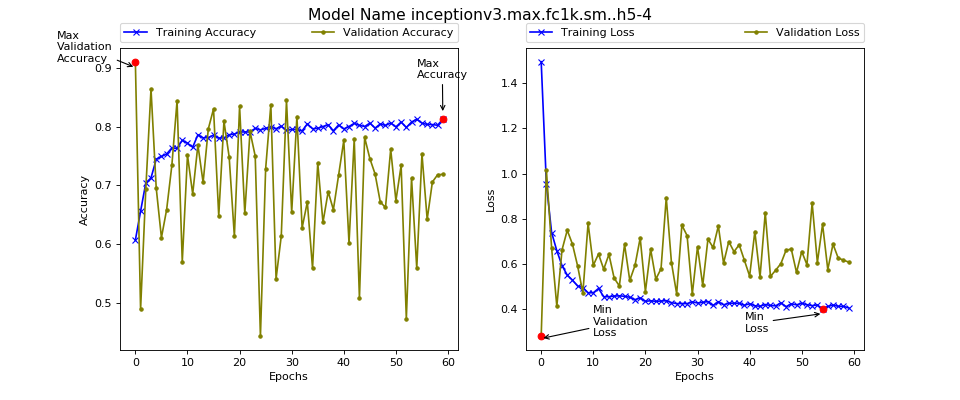
\includegraphics[scale=0.6]{images/t1-i3-fc1k-sm-4.png}
\caption{Inception Training Tasks Max Pooling Layer, FCN 1-layer 1024 and Softmax Classifier}
\end{figure}

The training procedure shows erratic validation training. Validation Accuracy immediately falls from the first epoch validation accuracy of 0.91. Learning rate is 1e-4, which could be too high for convergence. An average accuracy of value of 0.7 is acheived. The MaxPool layer shows a very erratic validation curve, whilst training curve increases gradually to a limit of 0.8. The MaxPooling layer will be dismissed.

\item: Inception with Global AveragePooling Layer and SoftMax Classifier
\begin{figure}[H]
\centering
\label{fig:incv3-gap-4}
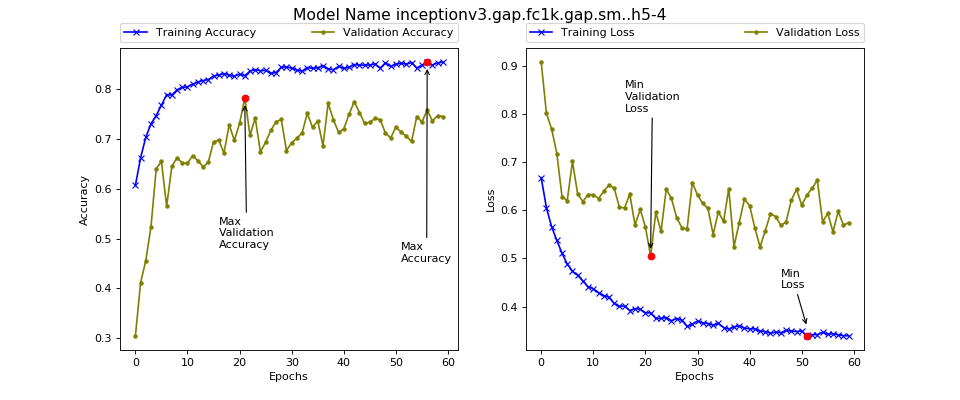
\includegraphics[scale=0.6]{images/t1-i3-gap-sm-4.png}
\caption{Inception Training Tasks GAP and Softmax Classifier - training Softmax layer}
\end{figure}

The InceptionV3 GAP layer maximum validation accuracy acheived when training on 4 layers, is of 0.781 accuracy at epoch 21. The number of trainable layers are increased to 37 layers, whilst using the same weights acheived earlier on. 

\begin{figure}[H]
\centering
\label{fig:incv3-gap-37}
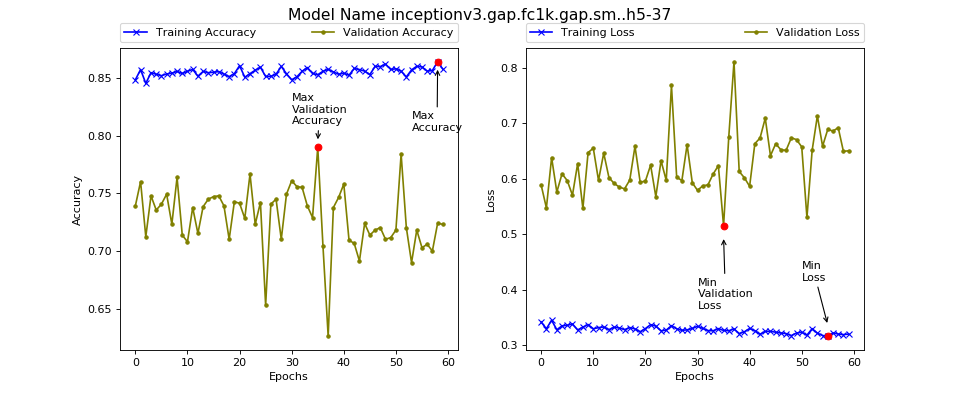
\includegraphics[scale=0.6]{images/t1-i3-gap-sm-37.png}
\caption{Inception Training Tasks GAP and Softmax Classifier - training last 37 layers}
\end{figure}

Validation accuracy increased to 0.79 at epoch 58. The number of trainable layers are increased to 37 layers.

\begin{figure}[H]
\centering
\label{fig:incv3-gap-65}
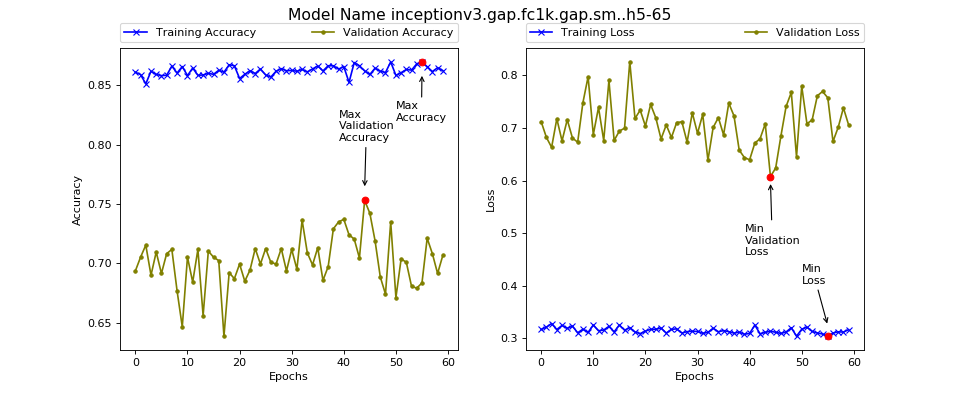
\includegraphics[scale=0.6]{images/t1-i3-gap-sm-65.png}
\caption{Inception Training Tasks GAP and Softmax Classifier - training last 65 layers}
\end{figure}

No further increase in accuracy has been noted, and the validation accuracy levels off at 0.7 mark average. To note the gradual improvement in training accuracy levels, during the training procedure , however the validation is more erratic. This shows a direct neural network to the convolutional output is unable to obtain the classifier features directly. The training accuracy levels off at a 0.87 mark, showing no increase during the last 120 epochs of the total 180 epochs run using a Global Average Pooling Layer. \newline

Incrementing the FCN to two layers produced an neural network without high value validation accuracy convergence.

\end{enumerate}
\subsubsection{Resnet-50}



\subsubsection{MobileNetv3}

A successful mobilenetv3 implementation will help us increase the speed of all subsequent inferencing. The default depth multiplier of 1 and default number of filters in the layer will be used as per paper. Detailed mobilenetv3 results are available in Appendix \ref{mobilenet}.

Mobilenetv3 test first using the Convolution Block and Softmax classifier directly to the two classes denoting foreground and background. The conv blocks and the classifier will be linked using Flatten or GlobalAveragePooling layer. Learning Rate 1e-5 used with RMSProp optimizer. Training Batch size 150 and Validation batch size 50. EarlyStopping is used as a regularizer with patience of 10 epoch training iterations. Results found in table \ref{mobilenetschedule}.

\begin{table}[ht]
\centering
\caption{Mobilenetv3 Training Schedule}
\label{mobilenetschedule}
\begin{tabular}{|l|l|l|} 
\hline
\textbf{MobileNetv3 architecture}                & \textbf{Maximum Accuracy }& \textbf{Epoch  }\\ 
\hline
Mobilenetv3+Flatten+SM                  & 0.8310           & 6      \\
Mobilenetv3+GAP+SM                      & 0.8233           & 55     \\
Mobilenetv3+GAP+FC1K+SM                 & 0.8442           & 12     \\
Mobilenetv3+GAP+FC2K+SM                 & 0.8674           & 10     \\
Mobilenetv3+GAP+FC4K+SM                 & 0.8645           & 15     \\
Mobilenetv3+GAP+FC2K+FC2K+SM            & 0.8188           & 50     \\
Mobilenetv3+GAP+FC2K+SM (conv13)        & 0.9514           & 50     \\
Mobilenetv3+GAP+FC2K+SM (conv12,conv13) & 0.9514           & 50     \\
\hline
\end{tabular}
\end{table}

The flatten layer in the first training gave an erratic training curve, so a GlobalAveragePooling layer was used for the rest of the schedule. A fully connected layer was introduced with varying widths (FC1K = 1024 neurons, FC2K = 2048 neurons and FC4K = 4096), followed by dropout layer at a rate of 0.5 and ending with a two-class softmax classifier(SM). The best accuracy achieved was for the Mobilenetv3+GAP+FC2K+SM. An extra hidden layer of 2048 did not improve accuracies. The only trainable layers were the Fully Connected Layers introduced, so the schedule started training the deepest convolutional block layers of Mobilenetv3. Training \textit{conv13 }and \textit{conv12+conv13 } resulted in the same maximum accuracy so no further testing were performed on the dataset.



\subsubsection{VGG-16}

\subsection{R-CNN Evaluation}

\subsubsection{Test 1: Sliding Window - Baseline}

Sliding Window uses the convolutional neural network over the whole image. Tiles of 224x224 size are cropped from original image from a 192 grid ($192 = 224-32$), with 32 being the overlap allowed between the two tiles to allow for detection of objects at the edge of the tile. The last row and last column are recalculated to allow for mismatching image height and width to grid. \newline

The tile passed to the VGG16 inferencing engine, which outputs a 2 unit tensor having values for [nolitter,litter]. The value of litter is stored in the detection grid. Bounding Box co-ordinates are obtained using tile co-ordinates for the tiles which inference results is higher than a preset confidence level. The bounding box predictions evaluated against the ground-truth values.\newline

VGG16 Training: A new VGG16 architecture will be trained on the dataset :dataset.v1. \textit{Conv5}, \textit{conv4} and \textit{conv4} will all have trainable layers. Two fully connected layers with relu activation and a softmax layer (2 classes) will be appended to the VGG16 convolutional layer output.
The CNN will be trained using checkpoint per epoch, early stopping based on Validation Accuracy metric with waiting for 10 epochs for validation accuracy improvement. 

\begin{table}[h]
\centering
\caption{Dataset.v1}
\begin{tabular}{lll}
\textbf{}  & \textbf{Litter} & \textbf{Background} \\
Training   & 5174            & 2672                \\
Validation & 208             & 1172               
\end{tabular}
\end{table}

Litter has been obtained from annotation data, whilst terrain obtained by sampling 10 images per scene, and vetted for presence of plastic or glass containers. Litter subdivided into 70\% training and 30\%  validation. However, 70\% training data has been augmented manually to 9 shifted positions.\newline

VGG16 architecture training: The validation accuracy obtained was of \textbf{0.9833}. \newline

\begin{table}[h]
\centering
\caption{Validation Class Report}
\begin{tabular}{lll}
\textbf{} & \textbf{Litter} & \textbf{Background} \\
Precision & 0.97            & 0.99                \\
Recall    & 0.95            & 0.99               
\end{tabular}
\end{table}

The precision/recall values are quite high for all the dataset. This maybe due to the limited number of cases present in the dataset. One has to note however that in RCNN the number of times the inference is done, where terrain is to be expected has a probability of 2000-3000 more than litter instances. Therefore the precision/recall obtained in the terrain 0.99/0.99 will have much more impact than the lower but less likely litter detection precision/recall  of 0.97/0.95.\newline

In a 4000 tile inference, 1\% of incorrect predictions would provide 40 False Positive predictions. In a typical scene 3 litter objects, would give us an R-CNN precision value of $\frac{3}{3+40} = 0.069$


Consumer Drone Testing Results: \textbf{Average Precision 0.14} at IoU of 0.1. The Recall rate is 0.922 (objects located within a bounding box) or 0.859 (bounding boxes predicting objects). Due to the large size of the bounding box with respect to the size of the detected object there are occasions of a bounding box covering two objects. Two recall rates are being reported to denote the descrepancy between the two possible calculations.\newline

This is a high recall rate indicating that litter is being detected successfully, and is very close to the validation litter rate detection.  However the precision rate is very small at \textbf{0.0586}, as per example above. 

\begin{enumerate}
\item Correct Predictions
\begin{figure}[H]
\centering
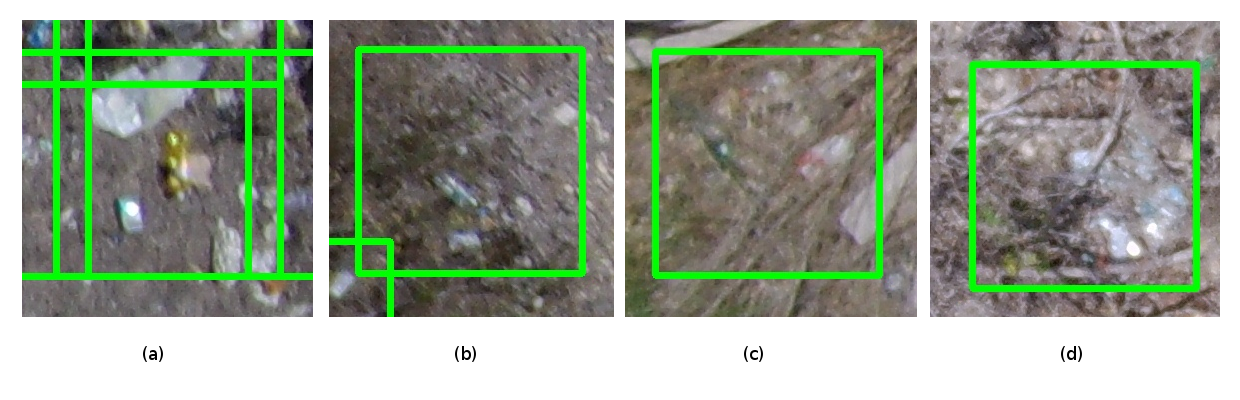
\includegraphics[scale=0.4]{images/test1-correct.png}
\caption{Sliding Window Correct Predictions}
\label{fig:test1correct}
\end{figure}

Figure \ref{fig:test1correct} shows successful predictions on the Consumer drone test set. The large sliding window size and stride do not hinder the correct inferencing. The ratio of the size of the detected object is comparable to the inferencing window. Figure \ref{fig:test1correct}c and \ref{fig:test1correct}d show occlusion and deformations being detected adequately. To denote the specular aspect of the objects being detected.

\item Incorrect Predictions But Plausible
\begin{figure}[H]
\centering
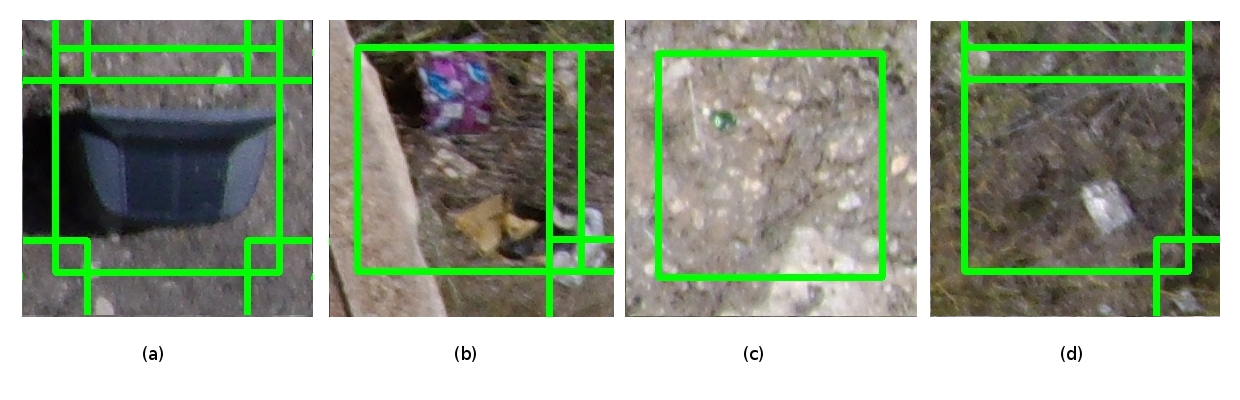
\includegraphics[scale=0.4]{images/test1-plausible.png}
\caption{Sliding Window Incorrect put Plausible Predictions}
\label{fig:test1plausible}
\end{figure}

Figure \ref{fig:test1plausible} shows a number of predictions that have not been annotated as beverage bottles, but which the algorithm has marked them as litter. These objects are frequent in the detected dataset. These artefacts found in outdoor imagery degrade the precision value, even though they could be successfully tagged as litter, though not beverage bottles or containers. The common aspect of these artefacts is that they are man-made objects, distinct from the background. Objects small as in figure \ref{fig:test1plausible}c are very frequent. However the ability to detect these small objects, although enhancing the shift invariance of the algorithm, can have a major detrimental effect on the precision value, as anything with this feature can be tagged incorrectly as litter. Such reflective objects could be stones, sea reflections, glass fragments, etc....Human annotations of these small objects is very difficult.

\item Incorrect Predictions that can be ammended
\begin{figure}[H]
\centering
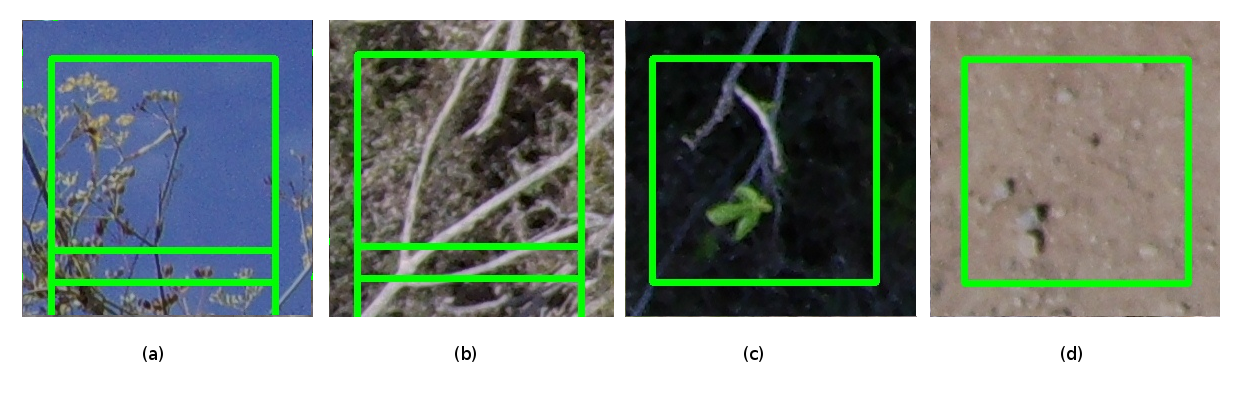
\includegraphics[scale=0.4]{images/test1-correctable.png}
\caption{Sliding Window Incorrect Predictions that could possibly be corrected}
\label{fig:test1correctable}
\end{figure}

Figure \ref{fig:test1correctable} shows example of uncorrect predictions that could possible by corrected. Figure \ref{fig:test1correctable}a shows a sky scene with branches that have been mistaken by the algorithm. This picture is evidently not an aerial image because sky can never be shown from a UAV with its camera shooting downwards. Accidental images such as these (during takeoff or landing of the drone) are possible and could be mistakenly placed within the dataset. The imagery can easily be removed by filtering \textit{sky} image tiles within the pictures. Figure \ref{fig:test1correctable} (b) and (c) are scenes  depicting vegetation and branches that also have been incorrectly misdetected. The regular features of the twigs could be affecting the CNN. However, different to the \textit{sky} images, plastic and litter can be found within \textit{vegetation} imagery, therefore handling vegetation must be done by the RCNN. Figure \ref{fig:test1correctable}d is an image with no clear plastic or man-made features. There is no clear explanation why the RCNN mistook this for litter. However, like \textit{vegetation} the RCNN could be trained to detect this type of imagery as terrain.

\begin{figure}[H]
\centering
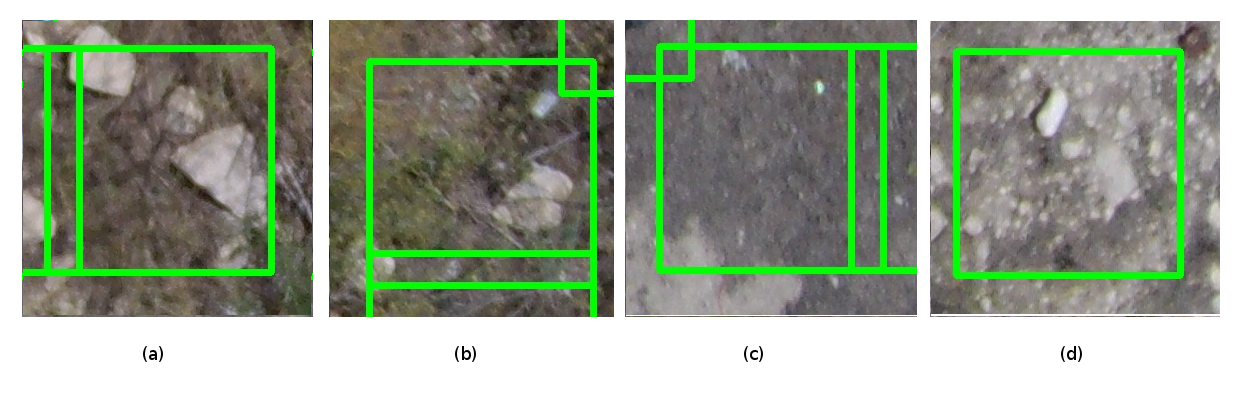
\includegraphics[scale=0.4]{images/test1-unkown.png}
\caption{Sliding Window Incorrect Predictions}
\label{figcorrectable2}
\end{figure}

Figure \ref{figcorrectable2}(a),(b) and (d) are images of stone incorrectly labelled as litter. Figure \ref{figcorrectable2}(d) particularly depict stones with a specular features and shapes very similar to plastic or glass bottles. Surprisingly some scenes contain a lot of these stones, to the detriment of the algorithm precision. Figure \ref{figcorrectable2}(c) shows a very small feature, as described  in figure \ref{fig:test1plausible}c affecting the classification of the CNN. This is caused by the high sensitivity to litter that has been designed within the dataset. Such example caused by high litter sensitivity will cause a high False Positive number. Unfortunately regular features can be detected anywhere within the outdoor imagery but not be result of manufacture but by stone formations or shadows. \newline
\end{enumerate}


GeoScience Drone Testing Results: \textbf{Average Precision 0.02} at IoU of 0.1. The recall rate is 0.896 (objects located within bounding box) or 0.8225 (bounding boxes predicting objects. The average precision is much lower than the consumer drone test results. The recall rate is lower but one can still say that out of the annotated number of bottles a good percentage is being detected. This indicates that the algorithm has a good degree of scale invariancy, since the statistics have shown that the size of the bounding boxes are different. The precision of the R-CNN is lowering the average precision value. At a precision rate of 0.0091 one can say that only 1 in 100 predictions is correct. This partly stems from the larger number of tiles to be predicted, and partly due to the new terrain which is causing the algorithm to wrongly detect litter.\newline 


\begin{enumerate}
\item Correct Predictions
\begin{figure}[H]
\centering
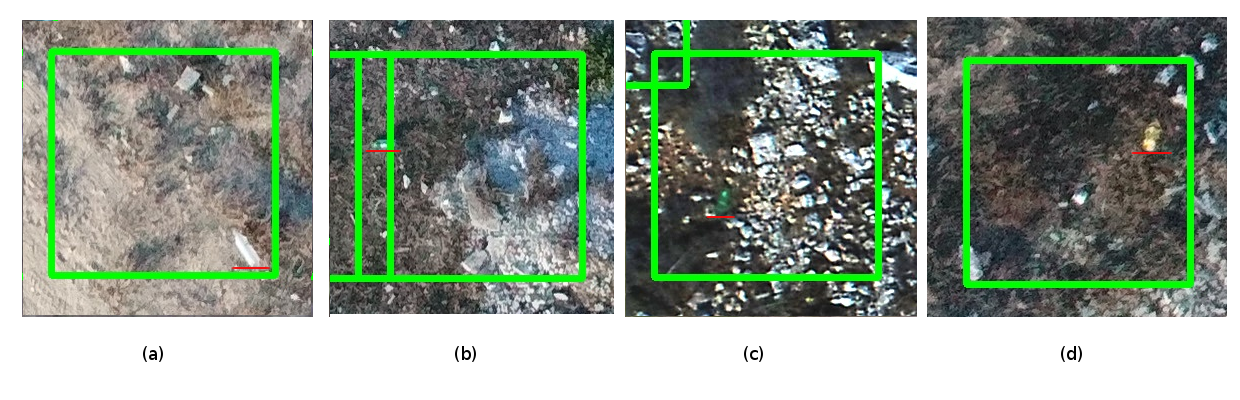
\includegraphics[scale=0.4]{images/test1-correct1.png}
\caption{Sliding Window Correct Predictions from GeoScience Survey}
\label{fig:correct2}
{\tiny The red underline is to highlight the position of the object}
\end{figure}

Figure \ref{fig:correct2} shows the correct predictions by the algorithm that have been detected. As expected the size of the objects are much smaller from the objects found in the Consumer database set. To note that the image quality is superior than the drone imagery, and the definitition of both the objects and the terrain is better. The quality difference might have an impact becuase of the regular features learnt by the CNN algorithm. The CNN is invariant of the position of the object, and the overlap in figure \ref{fig:correct2}(b) shows two nearby tiles detecting the same object.\newline


\item Incorrect Predictions but plausible
\begin{figure}[H]
\centering
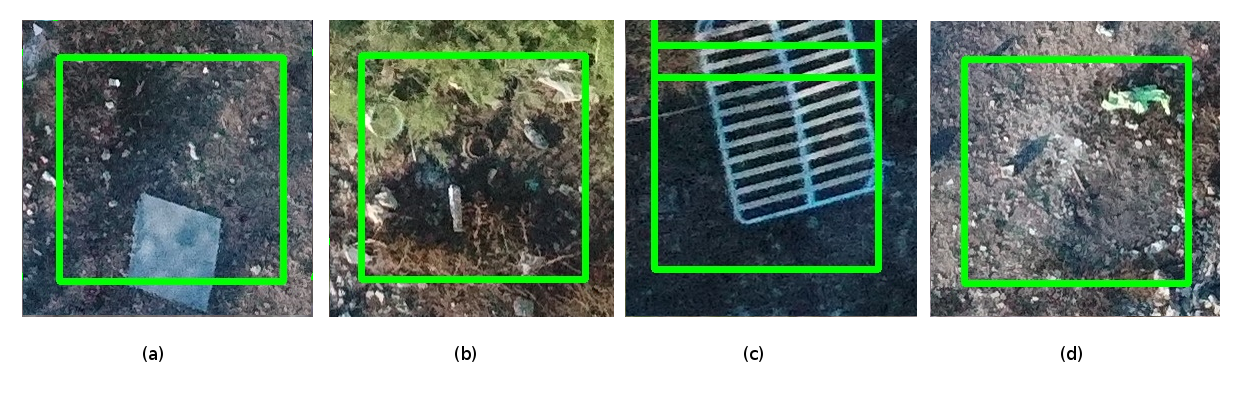
\includegraphics[scale=0.4]{images/test1-plausible1.png}
\caption{Sliding Window Incorrect but plausible predictions from GeoScience Survey}
\label{fig:plausible2}
\end{figure}

Here again we see that the algorithm is detecting very linear features and man-made shapes as being litter. Although one can correctly define them as litter the CNN algorithm was trained on beverage bottles and containers. The smooth and linear edges found within these objects are being extrapolated by the CNN as bottles. The CNN, as in case of \ref{fig:plausible2}(b) has managed to detect occluded objects. 

\item Incorrect Predictions that can be ammended
\begin{figure}[H]
\centering

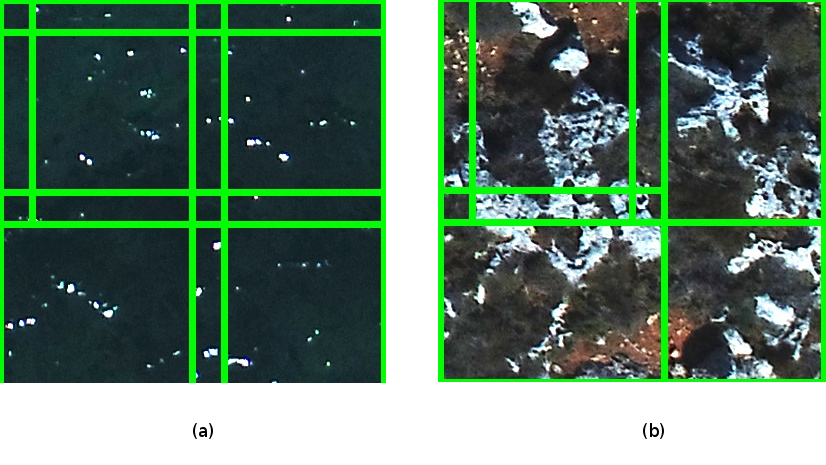
\includegraphics[scale=0.4]{images/test1-correctable2.png}
\caption{Sliding Window Incorrect predictions from GeoScience Survey (a) sea cover (b) rocky, grass and soil terrain}
\label{fig:correctable2}
\end{figure}

The geosciences dataset has a number of terrains not present in the consumer drone dataset. This has affected majorly the CNN inferencing ability on this dataset, why the precision rate for the GeoScience dataset is so low. The terrains in figure \ref{fig:correctable2} are an example of this imagery that are shown to be detected litter. Figure \ref{fig:correctable2}a is sea and the reflections on the ocean are being mistaken as specular reflections of bottles and glass. A large amount of incorrect predictions are being made, since the around 20\% of the survey is carried out over water. Since the application is for land-detection of litter, we can easily omit these by filtering these images out. With regards to \ref{fig:correctable2}b the CNN also is having a very large number of misdetections caused by unknown terrain. Removing such a terrain should be performed by modifying the litter detecting CNN, since plastic within this terrain should also be detected, and cannot be filtered out.

\end{enumerate}

\subsubsection{Comparison to other Small Object R-CNN}


\subsection{Test 2: Class Activation Mapping}

A human annotator will deduce the size of the objects once he starts reviewing the images from the aerial shots. The RCNN as shown is shift invariant to the cater very small objects as shown in figure \ref{fig:test1plausible}c and figure \ref{figcorrectable2}c. However, through Class Activation Mapping  one can determine the object size from CNN inference. A preliminary test on CAM methods has performed to compare it with the sliding window technique. The CAM 

\subsection{Test 3: Pre-Filter}

\subsection{Test 4: Dataset Engineering}

\subsection{Test 5: Field of View}

\subsection{Test 6: Further Data Augmentation}

\subsection{Test 7: Reduce Litter Sensitivity}

\subsection{Best R-CNN - AP vs size}

\subsection{Comparison with Peer Small Object Detection}

\textit{Indoor Objects}: Krishna et al \cite{Krishna} in their improving of small object detection data, improve on R-CNN by including an upsampling autoencoder with skip connections to upscale low-resolution data. The inferencing is done by a Faster RCNN with VGG16 algorithm. The dataset is based on internal scenes using internal objects, with a lesser degree of variability than outdoor terrain, and the CNN are trained to categorise the objects between themselves rather than a foreground/background technique used by the aerial-litter study.

\begin{table}[h]
\caption{Average Precision for the R-CNN and RPN using upscaling or superresolution, a subset of results}
\centering
\begin{tabular}{lllll}
\hline
\textbf{Method}                         & \textbf{Mouse}            & \textbf{Phone}            & \textbf{T.box}            & \textbf{Jar}             \\ \hline
\multicolumn{1}{|l|}{Faster R-CNN}      & \multicolumn{1}{l|}{57.7} & \multicolumn{1}{l|}{14.3} & \multicolumn{1}{l|}{8.1}  & \multicolumn{1}{l|}{3.1} \\ \hline
\multicolumn{1}{|l|}{RPN and upscaling} & \multicolumn{1}{l|}{56.8} & \multicolumn{1}{l|}{16.4} & \multicolumn{1}{l|}{23.4} & \multicolumn{1}{l|}{4.1} \\ \hline
RPN and superresolution                 & 60.1                      & 16.9                      & 12.8                      & 4.7                      \\ \hline
\end{tabular}
\end{table}

The litter dataset of 700 instances is close to the Average precision obtained for the tissue box at 100 instances. Krishna et al \cite{Krishna} mentions that 6000 instances are deemed a very small dataset that limits the ability to fine-tune the RCNN. To denote that our bi-linear upscaling of the image does not improve the average precision of either test or geoscience aerial-litter dataset. The litter detection smaller average precision number can be attributed to the foreground vs unlimited background, whereas this result is object vs object classification average precision.\newline

\textit{Traffic Signs}: Zhu et al \cite{Zhu2016} build an end-to-end CNN to detect and classify traffic signs. The signs. They report improvements in accuracy when data augmented with rotations between -20\degree and 20\degree. Something which we failed to see in our study. The dataset is based on 100000 scenes with 10,000 scenes containing 30,000 traffic signs, with images subdivided into theh COCO style image size categorisation of small (areas < $32^2$), medium (areas between $32^2$ and $96^2$) and large (area greater than $96^2$). They perform an easy filter by cropping 25\% top and 25\% bottom of the image since they presume no traffic signs will be located there. The comparison cannot be performed directly as the study relies only on recall values. They quote recall values of 0.24 for small objects, 0.74 for medium objects and 0.86 for large objects. In comparison, our RCNN fares very well with these values, as our recall values range from 0.82 to 0.9 for the datasets. Meng et al \cite{Meng2017} which use a similar sliding window approach to detect traffic signs. The dataset is based on 45 classes with more than 100 instances. The same size subsetting has been performed as Zhu et al\cite{Zhu2016}. The same recall-accuracy curves are obtained. \newline

The Feature Pyramid Network for small object detection by Lin et al \cite{Lin2017a} is trained on COCO dataset trainval35k and tested on the minival set. The dataset contains 80k training and 35k validation, segmented. The architecture uses a feature pyramid network for scale invariancy, using Fast RCNN approach with modified Resnet-50. We obtain results on par of their small objects (<32) for our objects which are to be considered medium. Again the foreground/background terrain problem does not appear to be present within this dataset. The results are shown in the table \ref{fpnresults}.

\begin{table}[]
\centering
\caption{Average Precision Results on COCO minival set}
\label{fpnresults}
\begin{tabular}{rccc}
\hline
\textbf{Fast R-CNN} & \textbf{AP\_\{s\}} & \multicolumn{1}{c|}{\textbf{AP\_\{m\}}} & \multicolumn{1}{c|}{\textbf{AP\_\{l\}}} \\ \hline
FPN                 & 0.178              & 0.377                                   & 0.458                                   \\
based on conv5      & 0.119              & 0.324                                   & 0.434                                   \\
based on conv4      & 0.157              & 0.365                                   & 0.455                                  
\end{tabular}
\end{table}

Atrous filter proposal by Guan et al \cite{Guan2017} does not specify the PASCAL VOC 2007 benchmark with a dataset being a mix of 16.5k images obtained from VOC2007 and VOC2012. The ARPN network uses a pyramid of filters to obtain different receptive fields. The AveragePrecision they quote is \textbf{0.114 for bottles} and 0.139 for plants, which is well on the par with our results.\newline

Eggert et al \cite{ChristianEggertStephanBrehmAntonWinschelDanZecha2017} on a dataset of logos from FlickrLogos dataset.  The paper proposes new anchors setups and RPN on standard VGG16 architecture, and then combine to an integrated detection pipeline. The FlickrLogos images within the dataset are distinct images of man-made bold illustration on backgrounds that enhance visibility. The results are as per table \ref{tableeggert}, show very high mean average precision values as a result. Our scene background is to the detriment of object visibility rather than enhancement.

\begin{table}[h]
\centering
\caption{Eggert et al \cite{ChristianEggertStephanBrehmAntonWinschelDanZecha2017} performance evaluation on FlickrLogos dataset}
\begin{tabular}{lll}
\hline
\textbf{Configuration}                              & \textbf{RPN MABO}         & \textbf{CLS (mAP)}        \\ \hline
\multicolumn{1}{|l|}{RPN performance}               & \multicolumn{1}{l|}{0.52} & \multicolumn{1}{l|}{0.51} \\ \hline
\multicolumn{1}{|l|}{RPN with original anchor sets} & \multicolumn{1}{l|}{0.66} & \multicolumn{1}{l|}{0.62} \\ \hline
\multicolumn{1}{|l|}{RPN with new anchor sets}      & \multicolumn{1}{l|}{0.68} & \multicolumn{1}{l|}{0.66} \\ \hline
\multicolumn{1}{|l|}RPN with multiple feature map and sets  & \multicolumn{1}{l|}{0.69                    } & \multicolumn{1}{l|}{0.66}
\end{tabular}
\end{table}

Another performance with a standard background is provided by the license plate recognition by Kim et al \cite{Kim2017}. The project uses DCNN which detects the presence of a number plate, the digits and the numbers within the same CNN architecture. The dataset was based on 200k postive images and 200k negative gray-scale images. DCNN achieves 0.993377 accuracy for license plate and 0.980266 for candidate regions. \newline

The Perceptual GAN for small object detection by Li et al \cite{Li2017} also attempt the traffic sign detection. Using a perceptual generative adversial approach with the generative branch based on a VGG16 network creates a super-resolved representation for the traffic sign. The discriminator network is a two branch network an adversarial branch to differentiate between the super-resolved feature and the original image, and the perception branch  to define accuracy. The architecture was tested on the PASCAL VOC2007 achieving an \textbf{AP of 0.694, 0.602, 0.579 and 0.418 } for boat, bottle, chair, and plant, respectively. This is much higher than our test results however the comparison of a multi-terrain imagery is still to be tested.\newline



\subsection{Comparison with Aerial Imagery Object Detection}

Literature review of small objects use a disparate methods of evaluation. Accuracy and background accuracy, total recall and total precision are used, so direct comparisons are problematic. Official datasets such as the VEDAI dataset \cite{razakarivony2016vehicle} where comparative results are published, there is a higher tendency to use official metrics such as AP. The background accuracy is a misleading accuracy as the number of tiles marked as background in large images is a large number. A very high accuracy rating would still be greater than the number of foreground annotations in an image with a very high foreground to background ratio.\newline

\subsubsection{Detection in Urban Environments}

Detection in urban environments make use of apriori knowledge of the urban background scenarios. Vehicle detection algorithms evaluated below use this knowledge to reduce the available search space. Methods replace RPN from Faster R-CNN to accomodate the distringuishing features of urban vs foreground images. \newline

Deng et al \cite{Deng2017} develop the AVPN for this purpose, using the Munich Vehicle dataset. AVPN selects from the image the best location where to look for a vehicle. Knowing that vehicles can only be located on roads and drive-ways,  the precision rate is as high as as 0.8593 for AVPN basic and 0.9198 for AVPNbasic + fast R-CNN. The recall rate is on par with our results of 0.7473 to 0.7702. At an IoU value of 0.2, the average precision obtained is 0.65 to 0.8 on sample of ten test images. The background/foreground discrimination ability of the algorithm on this dataset is the determining factor why it achieves this AP. \newline

The segment before detect approach as used by Audebert et al \cite{Audebert2017} use a SegNet a Segnet that produces semantic maps. The eroded regions obtained from the maps are sent to a vehicle detecting network based on LeNet, AlexNet and VGG-16. Regions of a default minimum size (as defined by the vehicle sizes seen) are removed. The author specifically remarks the improvement of evaluation scores when removing the small region areas. The data obtained from the VEDAI dataset \cite{razakarivony2016vehicle} containing detectable object of size $30 \times 30$. Various data augmentation techniques are  performed during training. Evaluation datasets used are VEDAI \cite{Razakarivony2015}, which are 1268 scenes ($1024 \times 1024$ pixels), ISPRS Potsdam 38 scenes ($6000 \times 6000$ pixels), and NZAM Christchurch 4 images ($5000 \times 4000$ size). Precision and recall results are obtained in table \ref{tablesegementeval}.

\begin{table}[h]
\centering
\caption{Vehicle detection results on the ISPRS Potsdam and NZAM/ONERA datasets}
\label{tablesegementeval}
\begin{tabular}{rcc}
\hline
\textbf{Dataset}                                                  & \multicolumn{1}{c|}{\textbf{Precision}} & \multicolumn{1}{c|}{\textbf{Recall}} \\ \hline
\begin{tabular}[c]{@{}r@{}}NZAM/ONERA\\ Christchurch\end{tabular} & 0.833                                   & 0.791                                \\
ISPRS Potsdam                                                     & 0.907                                   & 0.791                               
\end{tabular}
\end{table}

Zhong et al \cite{Zhong2017} also use the VEDAI dataset \cite{razakarivony2016vehicle} in their VPN implementation replacing the Faster R-CNN RPN filter. VPN uses multiple feature maps instead of just the final one (like RPN) and proposes areas where vehicles might be located. The network is based on a VGG-16 network. Results and comparison to other methods is shown in table \ref{zhongtable}.

\begin{table}[ht]
\centering
\caption{Results obtained by Zhong et al \cite{Zhong2017} using a VPN network proposal}
\label{zhongtable}
\begin{tabular}{rlccc}
\hline
\multicolumn{1}{|r|}{\textbf{Detection Model}} & \multicolumn{1}{l|}{\textbf{Image Size}} & \multicolumn{1}{c|}{\textbf{Recall}} & \multicolumn{1}{c|}{\textbf{AP}} & \multicolumn{1}{c|}{\textbf{F1-Score}} \\ \hline
Faster R-CNN (Z\&F)                            & 1024 x 1024                              & 0.635                                & 0.308                            & .0229                                  \\
Faster R-CNN (VGG-16)                          & 1024 x 1024                              & 0.739                                & 0.421                            & 0.232                                  \\
Fast R-CNN (VGG-16)                            & 1024 x 1024                              & 0.722                                & 0.398                            & 0.216                                  \\
SLIC with Z\&F                                 & 1024 x 1024                              & 0.583                                & 0.254                            & 0.066                                  \\
SLIC with VGG-16                               & 1024 x 1024                              & 0.588                                & 0.232                            & 0.064                                  \\
Our Model                                      & 1024 x 1024                              & 0.723                                & 0.546                            & 0.320                                  \\
Faster R-CNN (Z\&F)                            & 512 x 512                                & 0.609                                & 0.320                            & 0.212                                  \\
Faster R-CNN (VGG16)                           & 512 x 512                                & 0.714                                & 0.409                            & 0.225                                  \\
Fast R-CNN(VGG16)                              & 512 x 512                                & 0.694                                & 0.373                            & 0.224                                  \\
Our Model                                      & 512 x 512                                & 0.697                                & 0.502                            & 0.308                                 
\end{tabular}
\end{table}

The table \cite{Zhong2017} shows that a Faster R-CNN used within this type of application acheives an AP of 0.308. With such a comparably small recall one should note that the AP is being augmented primarily by the precision obtained. The task at hand shows that the RCNN has high discrimintary features that enhances the vehicle detection accuracies obtained.\newline 


Ammour et al \cite{Ammour2017} using the same UAV surveying technologoy for vehicle detection, uses mean-shift algorithm to segment the image into regions of the same HSV value. The classifier is based on a VGG16 architecture with an SVM classifier. Again a selection of regions is performed depending on size, with operations on the resultant mask to fill small holes, mask dilation and inspecting isolated regions. The regions were tuned by Meanshift to cover roughly one-tenth of the car, which would cover the different car features such as windscreen, roof, backscreen, side doors, etc... The results shown in table \ref{meanshiftveh}.

\begin{table}[ht]
\centering
\caption{Ammour et al \cite{Ammour2017} detection results for vehicle detection using Mean-Shift}
\label{meanshiftveh}
\begin{tabular}{lcccll}
\textbf{Test Image} & \textbf{Cars Present} & \textbf{TP} & \textbf{FP} & \textbf{Recall} & \textbf{Precision} \\
Image 1             & 56                    & 47          & 4           & 0.839           & 0.922              \\
Image 2             & 31                    & 26          & 10          & 0.839           & 0.722              \\
Image 3             & 19                    & 14          & 7           & 0.737           & 0.667              \\
Image 4             & 16                    & 13          & 0           & 0.813           & 1.000              \\
Image 5             & 5                     & 4           & 2           & 0.800           & 0.667             
\end{tabular}
\end{table}

Different to vehicle detection but still using the urban environment distinguishing features is the Solar Photovoltaic Array Detection as studied by Malof et al\cite{Malof2016}. The algorithm uses an ensemble of Random Forest and CNN algorithms. The RF prescreens the object locations and CNN detect the PV panels. The input image is to the CNN is a $40 \times 40$ image. The algorithm achieves a recall of 0.9. The precision recall curve is shown in figure \ref{curvepanel}.

\begin{figure}[h]
\centering
\label{curvepanel}
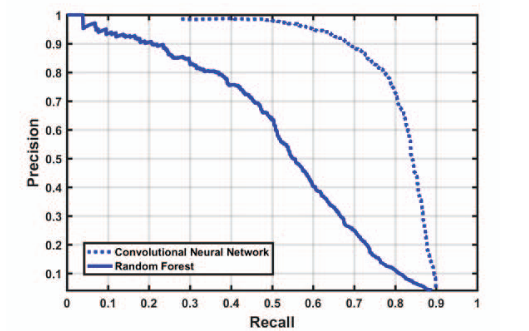
\includegraphics[scale=0.4]{images/pvpanels.png}
\caption{Precision Recall curve of RF/CNN panel detection by Malof et al \cite{Malof2016}}
\end{figure}


\subsubsection{Other Aerial use of CNN}

Other Aerial imagery applications do not have the urban environment of the vehicle detection, however most studies fail to mention the problematics of the high variable in the background. One should deduce that the studies did not encounter problems with the variable background.\newline

The fast animal UAV detection by Kellenberger \cite{Kellenberger2017} uses 654 images from the SAVMAP project, from the Kuzikus Wildlife reserve park in Namibia. Kellenberger reduces the IoU threshold to 0.25 (as for all small object detection methods). The pre-trained Alexnet used is trained on animals against background. Improvments on the CNN is a two-branch approach that also calculates the size of the objects detected as a classifying feature. No mention of the type of backgrounds in the images is mentioned. Results shown in table \ref{tablekellen}. 

\begin{table}[ht]
\centering
\caption{Results for Fast UAV detection of animals by Kellenberger et al \cite{Kellenberger2017}}
\label{tablekellen}
\begin{tabular}{lcc}
\textbf{}                            & \textbf{Fast R-CNN (baseline)} & \textbf{Proposed Model} \\
Ground-Truth Objects                 & 509                            & 509                     \\
True Positives                       & 429                            & 379                     \\
\multicolumn{1}{l|}{False Positives} & 843                            & 254                     \\
False Negatives                      & 80                             & 130                     \\
Precision                            & 0.34                           & 0.60                    \\
Recall                               & 0.84                           & 0.74                    \\
F1-Score                             & 0.48                           & 0.66                   
\end{tabular}
\end{table}

Another aerial imagery use of CNN algorithms in ecological projects, is the detection of white geese by Bowley et al \cite{Bowley2017}. The study identifies the problematics of background variability, and stresses the importance the use of a lot of data. In fact Bowley et al \cite{Bowley2017} use a dataset of 65,000 annotated images. Very high altitudes were used, for geese detection, using a 16Mpixel camera. The CNN used an image detection of $18 x 18$ pixel, since the end objects were of 14 - 18 pixels in width/height. A custom CNN used with 2 convolutional layers and 2 fully connected layers. Training was done of white geese versus background. The results obtained are shown in table \ref{whitegeese}.

\begin{table}[ht]
\centering
\caption{Testing Accuracy Results obtained by Bowley et al \cite{Bowley2017} }
\label{whitegeese}
\begin{tabular}{rccc}
\textbf{CNN} & \textbf{\begin{tabular}[c]{@{}c@{}}White Phase\\ (geese)\end{tabular}} & \textbf{Background} & \textbf{Total} \\
Expert       & 0.9626                                                                 & 0.9991              & 0.9981         \\
Matched      & 0.9152                                                                 & 0.9995              & 0.9976         \\
Unmatched    & 0.9526                                                                 & 0.9975              & 0.9964        
\end{tabular}
\end{table}

Matched observations are the joint annotations done by both experts and citizens. An error rate of 0.9995 on a $3000 \times 2000$ image creates 9 False Positive per scene, which is not such a distant metric than that obtained by the aerial litter detection method.


Avalanche search and rescue project for real-time object detection by a UAV, is an CNN application studied by Begija et al \cite{Bejiga2016} uses a pretrained GoogleNet \cite{Szegedy2015} but with an SVM classifier. A sliding window approach is used on $224 \times 224$ tiles. The results report is in the form of $P_{FA}$ (probability of negative samples) and $P_{TP}$ (probability of positive samples). This can be misleading because the $P_{FA}$ against the whole background can result in a significant amount of tiles. The results are shown in table \ref{skiing}. 

\begin{table}[ht]
\centering
\caption{Classification Results of Avalanche Search and Rescue by Bejiga et al \cite{Bejiga2016}}
\label{skiing}
\begin{tabular}{llll}
\textbf{}                                                 & \textbf{Accuracy} & \textbf{$P_{FA}$} & \textbf{$P_{TP}$} \\
Downsample of whole image to $224 \times 224$             & 0.6571            & 0.5283          & 0.8462          \\
Downsample of $672 \times 448$ tiles to  $224 \times 224$ & 0.9429            & 0.1095          & 0.6346          \\
Sliding Window                                            & 0.9759            & 0.0152          & 0.8065         
\end{tabular}
\end{table}

\subsection{Evaluation Conclusion}

Comparing the aerial-litter detection results from the results obtained in the literature we find that the recall values are on the par with many papers, and some exceeding the detections available. However high recall with no precision is useless. A problem with our evaluation is our imposed limitation with respect to object we required identification. The CNN is able to find many more litter instances such as boots, paper/cartoon, plastic bags, cloth, etc... that would have increased the Average Precision values obtained. \newline

When comparing the algorithm to a generic small object detection such as that of Krishna et al \cite{Krishna} we find that the RCNN has the same range of average precision values. Traffic signs, vehicles in an urban environment, logos etc... have a high discriminatary features between foreground and background, that makes the evaluation against these problems not comparable. The segmentation ability of the background within this vehicle detection evaluation is a clear marker of precision values obtained with a known background filter, such as a segmentation CNN pre-filter. This tallies with our pre-filter which achieved an increase in precision values within both of the datasets. However, the removal of specific backgrounds is impossible with the aerial-litter detection, as litter can be found anywhere on land. Therefore no land or land-type can be removed without reducing the recall values obtained. Vehicle detection and solar panels have another advantage of being highly homongenuous in size, shape and colour.\newline

A common aspect of the evaluation papers is the availability of large annotated datasets and default evaluation methods. In the review of these papers, the evaluation vary a lot making comparisons between them hard enough. We used a default PASCAL VOC 2012 evaluation criters. The size of our dataset is small due to the time constraints that limited data gathering and annotation. As can be seen from our tests whenever more raw data was included in the dataset our Average Precision got better. Data Augmentation is not a substitute for raw data as the iterations and permutations found in real-world imagery cannot be replicated using mathematical transformation. \newline

\section{Future Works}

\begin{enumerate}
\item More Data - Increase terrains and sensors
\item Embedded CNN - GAP for proposals (image shape and size) + detector
\item Use of Shallower layers in the GAP VGG architecture
\item Custom-made CNN with learning from scratch - 
\item Custom made with one size input layer based on image size
\item Automatic Object size Detection
\item Automatic dataset generation using Human Confirmation
\end{enumerate}

\appendix

\subsection{Mobilenetv3 Training and Testing on Dataset v3}
\label{mobilenet}


\bibliographystyle{IEEEtran}
\bibliography{mybib}

\end{document}

